\section{Evaluation}\label{sec:evaluation}

\subsection{Data inputs}

\textit{We discuss how an attacker can inject arbitrary bytes into receivers.  We measure the effectiveness of this approach by an overshadowing simulation.  We discuss how data can also be inserted through the mailing list}

\subsection{Security audit}
\textit{Table demonstrating which currently-active CVEs are present in the software. A discussion of legacy software and its relation to security}

\subsection{Radio link evaluation}
\textit{Simulated measurements showing how successful an attacker could be in overshadowing the radio signal with their own}

%The proposed evaluation would consist of several stages:

%\begin{itemize}
    %\item A demonstration of calculating the phase cancelling and injecting signal from an arbitrary image
    %\item An evaluation of how often an attacker's receiver station can reliably decode the transmission well enough to perform signal injection
    %\item A demonstration that, given the direct playback transmission, a receiver can successfully synchronise and inject the signal at the right time
    %\item An end-to-end demonstration that the spoofed image can be injected, and then fool the FIRMS forest fire detection algorithm
%\end{itemize}

\begin{figure}
    \centering
    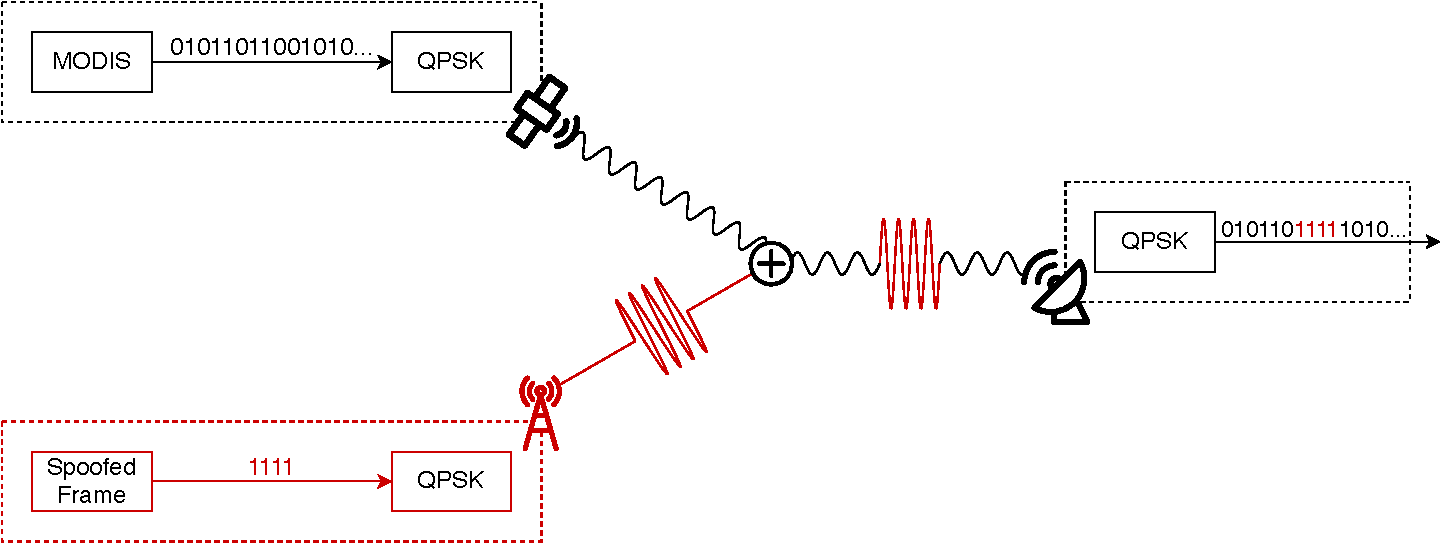
\includegraphics[width=\columnwidth]{diagrams/overshadowing_demo.pdf}
    \caption{Representation of a signal injection attack through overshadowing.}
    \label{fig:overshadowing_demo}
\end{figure}

In order to demonstrate the feasibility of signal injection through overshadowing in a real-world setting, we construct an end-to-end software pipeline to demonstrate the attack.
This pipeline, built using ``GNU Radio'', encodes the victim's signal using the QPSK modulation pipeline described in \textbf{TODO}.
An attacker's signal is also encoded and amplified by a specified amount.
At a specified time this signal is injected on top of the victim's signal by adding the samples together, mimicking the behaviour of a radio receiver picking up the two superimposed signals.
A QPSK demodulation pipeline outputs the resulting bytes.
This is illustrated in Fig.~\ref{fig:overshadowing_demo}.

We measure the performance of a given configuration by looking for the frame header bytes in the decoded signal -- these indicate the attacker was successfully able to inject a frame.
For each configuration we repeat the attack 1024 times to get an overall success rate for that configuration.
We measure success rate for varying levels of background noise, and power of the attacker's signal.
Signal-to-noise ratio (SNR) is computed from the victim signal using the following:

\begin{equation}
\label{eq:snr}
    \text{SNR} = \frac{\text{signal amplitude}^2}{\text{noise amplitude}^2}
\end{equation}

\begin{figure*}
    \centering
    \begin{subfigure}{0.95\columnwidth}
        \centering
        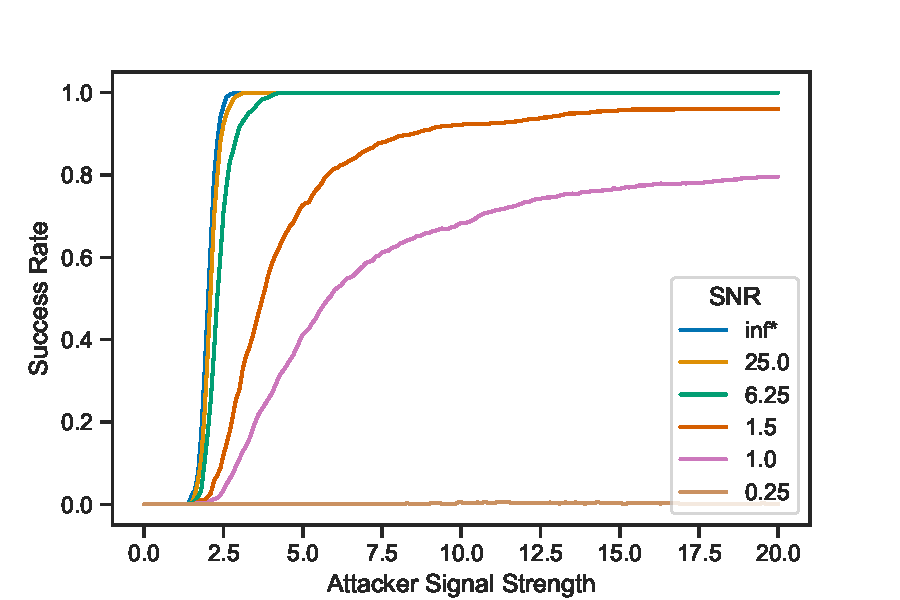
\includegraphics[width=\columnwidth]{diagrams/attack_strength.pdf}
        \caption{Success rate as signal strength increases, for a range of SNRs.\\\footnotesize{\normalfont{*no noise on channel}}}
        \label{fig:attack_strength}
    \end{subfigure}
    \hfill
    \begin{subfigure}{0.95\columnwidth}
        \centering
        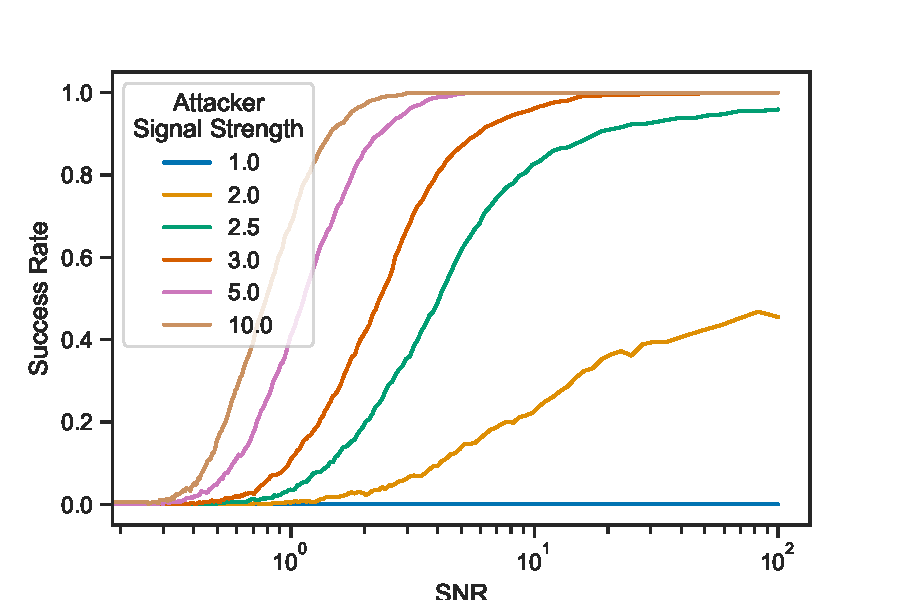
\includegraphics[width=\columnwidth]{diagrams/attack_snr.pdf}
        \caption{Success rate as SNR increases, for a range of signal strength values.}
        \label{fig:attack_snr}
    \end{subfigure}
    \caption{Success rate of signal overshadowing. Signal strength given as a multiple of victim signal strength.}
\end{figure*}


Fig.~\ref{fig:attack_strength} illustrates the success rate of the attack as we increase the power of the attacker's signal for a range of background noise levels.
Similarly, Fig~\ref{fig:attack_snr} shows the success rate of the attack for various attacker power levels, as we vary the noise on the receiver.
It is clear that with low to moderate levels of noise the success rate of the attack eventually reaches 100\%.
By measuring the noise level at the receiver and consulting this figure, the attacker can derive the minimum transmission power required (relative to the victim signal) to overshadow the signal with a maximal success rate.
When noise is low, the signal needs to be roughly $2.5$~times as strong as the victim signal.
Above a certain noise level, the success rate of the attack is unable to reach 100\% -- with this much noise on the channel, not even a legitimate signal is able to get through.
